\documentclass{amsart} 
\usepackage{amsmath}
\DeclareMathOperator*{\argmax}{arg\,max}
\DeclareMathOperator*{\argmin}{arg\,min}
\usepackage{graphicx}
\graphicspath{{./}}
\usepackage[fontsize=14pt]{scrextend}
\usepackage{hyperref}
\usepackage{csvsimple}
\usepackage{epigraph}
\title{Happiness Prediction Explaining 50 Percent of Variation}
\author{Zulfikar Moinuddin Ahmed}
\date{\today}

\begin{document}
\maketitle
\epigraph{You are not to blame for

Bittersweet distractors

Dare not speak its name

Dedicated to all human beings

Because we separate

Like ripples on a blank shore

In rainbows

Because we separate

Like ripples on a blank shore

Reckoner

Take me with you

Dedicated to all human beings}{Radiohead, "Reckoner"}

\section{The Focus is on Universality}

One of the most difficult tasks for human beings when addressing issues of Human Nature had always been to produce clear truth regarding features that are both {\em nontrivial} and {\em nation-language-culture-religion-ethnicity independent}.  It has been so difficult that there are very rare acceptance that almost {\em anything at all} has universality that crosses all national, cultural, ethnic, linguistic boundaries.  Often, there is even {\em conviction} that no nontrivial universality exists not just in the West but also in the East, that all important features of human beings are permanently and indelibly and deeply marked by nation-culture-language-ethnicity-religion.  This is an example of a strong solid result that is universal.  I am predicting happiness across the world with fairly clear and uncomplicated measurements with $R^2=0.5$ which is very good for Social Science.  This matters a great deal because we are paralysed by issues of racial differentiation, ethnic strife in America and elsewhere, and exhortations by people like myself for acceptance of a single human race as a deep absolute truth are dismissed as 'politically correct' and such things.  Here you will see concrete and clear strong result that nontrivial universal results are clear and strong and not a result of political chicanery.


\section{Precise Meaning of Happiness}

We consider the combined total percent of countries falling in category "very happy" and "happy" as our metric of happiness.  We have to be precise because we are trying to understand finer issues of noise and so on and at the moment we don't know if a different measure would be quite different in characteristics.

\section{Result}

\begin{verbatim}
== Log linear
> summary(mod.hapcor)

Call:
lm(formula = log(happy + 1) ~
 log(trustMost + 1) + 
 log(Autonomy + 1) + 
 log(finsat + 1), data = hapcor)

Residuals:
      Min        1Q    Median        3Q       Max 
-0.307873 -0.035315  0.007082  0.045083  0.130870 

Coefficients:
                   Estimate Std. Error t value Pr(>|t|)    
(Intercept)         3.32201    0.13696  24.256  < 2e-16 ***
log(trustMost + 1)  0.06793    0.01650   4.118 9.73e-05 ***
log(Autonomy + 1)  -0.03606    0.01510  -2.388   0.0195 *  
log(finsat + 1)     0.24687    0.03484   7.086 6.42e-10 ***
---
Signif. codes:  0 ‘***’ 0.001 ‘**’ 0.01 ‘*’ 0.05 ‘.’ 0.1 ‘ ’ 1

Residual standard error: 0.07266 on 75 degrees of freedom
Multiple R-squared:  0.5268,	Adjusted R-squared:  0.5078 
F-statistic: 27.83 on 3 and 75 DF,  p-value: 3.347e-12
\end{verbatim}

In order to assess the quality of the prediction, we have this graphical display of measured versus predicted log-happiness.

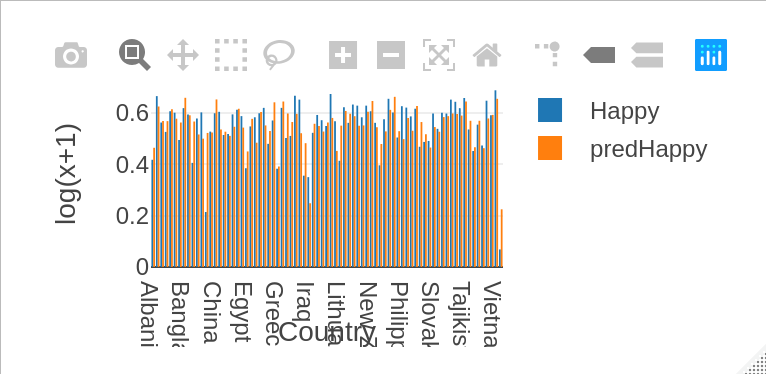
\includegraphics[scale=0.8]{predhap.png}

\section{Residual Noise}

The residual noise in the above model shows nontrivial gamma and other non-Gaussian parameters in Generalised Hyperbolic Distribution.

\begin{verbatim}
Asymmetric Generalized Hyperbolic Distribution:

Parameters:
   lambda alpha.bar        mu
-3.713144  1.512722  5.592804               
   sigma     gamma 
6.019867 -5.526398 

Call:
fit.ghypuv(data = mod.hapcor$residuals * 100)

Optimization information:
log-Likelihood:                -260.7763 
AIC:                           531.5527 
\end{verbatim}


\end{document}
